\documentclass[10pt,twocolumn]{article} 
\usepackage{simpleConference}
\usepackage{fancyhdr}
\usepackage{amsmath,amsfonts,amssymb,graphicx}
\usepackage{subfigure}   % 使用子图形
\usepackage{indentfirst} % 中文段落首行缩进
\usepackage{bm}          % 公式中的粗体字符(用命令\boldsymbol)
\usepackage{indentfirst} % 中文首段缩进
\usepackage{abstract}    % 2栏文档,一栏摘要及关键字宏包
\usepackage{amsthm}      % 使用定理
\usepackage{booktabs}    % 使用表格
\usepackage{siunitx}
\usepackage{tikz}
\usepackage{titlesec}
\usepackage{times}
\usepackage{wasysym}
\usepackage{pifont}
\usepackage{ccaption}
\usepackage{float}
\usepackage{calc}
\usetikzlibrary{calc}
\usetikzlibrary{circuits.ee.IEC}
% 在导言区添加 circuitikz 包
\usepackage{circuitikz}
\usepackage{environ}
\usepackage{lmodern}
\usepackage{anyfontsize}
\usepackage{hyperref}
\usepackage{tabu}
\usepackage{tabularx}
\usepackage{multirow}
\usepackage{multicol}
\usepackage{longtable}
\usepackage{makecell}
\usepackage{graphicx}
\usepackage{amssymb}
\usepackage{url,hyperref}

\newcommand*{\effXsecDPS}{\sigma_{\text{eff,DPS}}}
\newcommand*{\effXsecTPS}{\sigma_{\text{eff,TPS}}}

\begin{document}

\title{Search for Simultaneous Production of Double $J/\psi$ and $\Upsilon$ Mesons,\\Double $J/\psi$ and $\phi$ Mesons, or $J/\psi$, $\Upsilon$ and $\phi$ Mesons in Proton-Proton\\ Collisions at $\sqrt{s} = 13.6 ~ \mathrm{TeV}$ at the CMS Experiment}

\author{Chi Wang \\
\\
Topics on Frontiers of Cross-Sciences Course Report \\
Zhili College, Tsinghua University, China \\
\today
\\
\\
chi.w@cern.ch  \\
}

\maketitle
\thispagestyle{empty}

\begin{abstract}
The material in this template is an edited \& \LaTeX\--ified version of the recommendations here: \url{http://cs.stanford.edu/people/widom/paper-writing.html} The objective would be to help us writers, stay on topic and focused for each section of a report.

For the abstract state the problem, your approach and solution, and the main contributions of the paper. Include little if any background and motivation. Be factual but comprehensive. The material in the abstract should not be repeated later word for word in the paper. 
\end{abstract}


\section{Introduction}

\subsection{Multi-Parton Scattering in Proton-Proton Collisions}

Proton consists of three quarks, two up-type and one down-type, and gluons, which hold together the three valence quarks, as well as of a ‘sea’ of virtual quark–antiquark pairs. All these components are referred to as ‘partons’, with point-like behaviour in deep inelastic scatterings.\cite{}

In the standard picture of proton–proton (pp) collisions, typically only a few partons undergo a hard scattering with one another, with the remainders of each proton only slightly disturbed in the process. As the collision energy increases, the densities of gluons and sea quarks probed inside each proton grow rapidly. Thus, at higher collision energies, it becomes more likely for more than one pair of partons undergo a hard scattering in a single pp collision, leading to the simultaneous and independent production of two or more particles with transverse momentum ($p_T$) and/or mass ($m$) above a few giga-electronvolts. Such processes are collectively referred to as multi-parton scattering (MPS).

MPS processes offer an important probe into the complicated inner structure of the proton and its evolution with energy.\cite{DIEHL_MPI}\cite{BLOK_MPS} Many of these features, for example, the parton density profile in the plane transverse to the colliding beams, as well as the various correlations (in position, momentum, flavour, colour, spin and so on) between individual partons, are very difficult to calculate theoretically, since , and can only be mapped out through experimental studies of MPS in different systems and for different numbers $n$ of simultaneous scatterings \cite{MPI_LHC}.

In addition to providing an insight into proton structure, MPS studies also contributes to background subtraction in future searches for rare standard model and beyond-standard model resonances, especially at future hadron colliders, where the MPS contribution to the backgound becomes more significant due to higher centre-of-mass energy.\cite{DdE_TPS}\cite{YJZ_TRI_JPSI}

\subsection{The "Pocket Formula" and $\sigma_{\text{eff,NPS}}$}

Under the most simple assumption that the individual sub-scatterings are independent, one may consider the probability for the multiple production of particles with a high transverse momentum proportional to the product of the probabilities for each individual sub-scattering. This relation is more commonly expressed in terms of cross sections as the "pocket formula" shown below, for an arbitrary number $n$ of sub-scatterings:

\begin{equation}
\begin{aligned}
    \label{eqn:nps_pocket}
    &\sigma^{pp\to\psi_1+\psi_2+\cdots+\psi_n+X}_{\text{NPS}} \\&=
    \left(\frac {\mathfrak{m}}{n!}\right) \frac{\sigma_{\text{SPS}}^{pp\to \psi_1+X}\sigma_{\text{SPS}}^{pp\to \psi_2+X}\cdots\sigma_{\text{SPS}}^{pp\to \psi_n+X}}{(\sigma_{\text{eff,NPS}})^{n-1}}
\end{aligned}
\end{equation}

In the "pocket formula" (eqn. \ref{eqn:nps_pocket}), the effective cross section $\sigma_{\text{eff,NPS}}$ is only determined by the transverse parton density overlap, and the combinatorial factor $\mathfrak{m}$ is used to remove the duplicate counting from same-type particle final states.

Double parton scattering (DPS) processes are the most trivial MPS processes and the first observed. The first observation of DPS processes was made by the AFS collaboration on the Intersecting Storage Ring (ISR) at CERN\cite{ISR_DPS}. Since then, a variety of DPS processes have been studied on high-energy hadron colliders such as the Tevatron and the Large Hadron Collider (LHC).

In DPS processes, the "pocket formula" (eqn. \ref{eqn:nps_pocket}) can be more specifically written with the expression below:

\begin{equation}
\begin{aligned}
    \label{eqn:dps_pocket}
    \sigma^{pp\to\psi_1+\psi_2+X}_{\text{DPS}}=
    \left(\frac {\mathfrak{m}}{2!}\right) \frac{\sigma_{\text{SPS}}^{pp\to \psi_1+X}\sigma_{\text{SPS}}^{pp\to \psi_2+X}}{\effXsecDPS}
\end{aligned}
\end{equation}

From the proton forms adopted by event generators like Pythia8 and Herwig++, it is expected that the $\sigma_\text{eff,DPS}$ would fall in the range of $20 \to 30~\mathrm{mb}$ and would not depend on the final state studies. However, as summarized in figure \ref{fig:sigma-eff-dps-summary}, $\sigma_\text{eff,DPS}$ results obtained from experiments have been much lower, with $\sigma_\text{eff,DPS}\approx 10-20~\text{mb}$ from final states containing jets and/or electroweak bosons\cite{ATLAS_4JET_7TEV}\cite{ATLAS_WJetJet_7TEV}\cite{ATLAS_Z_JPSI}\cite{CDF_4JET}\cite{CMS_4JET_13TEV}\cite{CMS_WJETJET_7TEV}\cite{CMS_WW_DPS_8TEV_LIM}\cite{CMS_WW_DPS_13TEV_FOUND}, and even lower values of $\sigma_\text{eff,DPS}\approx 3-10~\text{mb}$ extracted from processes where two heavy quarkonia like $J/\psi$ and $\Upsilon$ are produced\cite{ATLAS_JPSIJPSI_8TEV}\cite{ATLAS_JPSI_PSI2S_7_8_TEV_COMBINED}\cite{CMS_INCL_JPSIJPSI_7TEV}\cite{ CMS_JPSIPSI2S_7TEV}\cite{CMS_JPSIPSI2S_DIFF_7TEV}\cite{CMS_YY_8TEV}\cite{CMS_YY_XSEC}.

\begin{figure}[H]
    \centering
    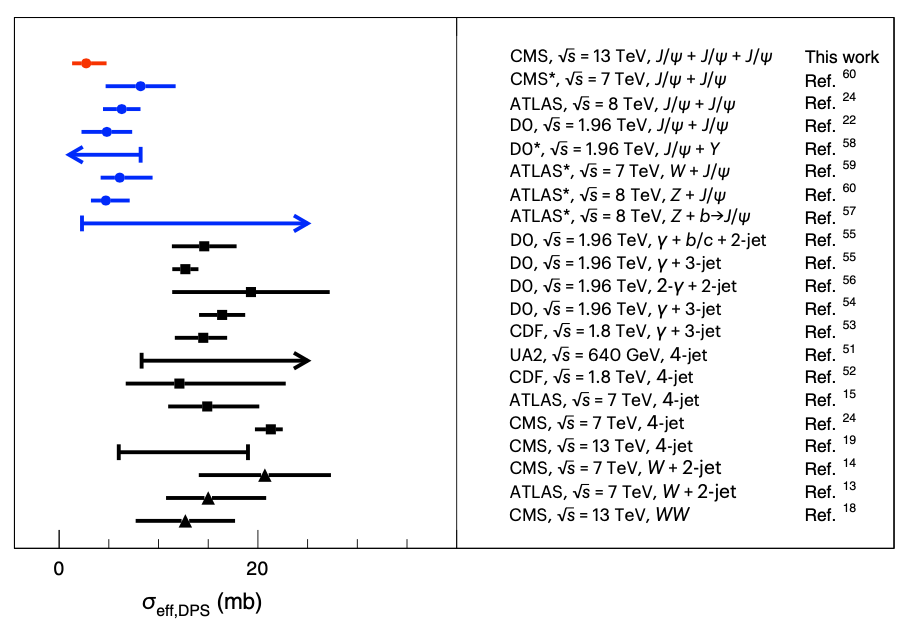
\includegraphics[width=1.0\linewidth]{images/sigma_eff_DPS_summary.png}
    \caption{Summary of current $\effXsecDPS$ measurement results in various final states\cite{CMS_TRI_JPSI}}
    \label{fig:sigma-eff-dps-summary}
\end{figure}

Disagreement in $\effXsecDPS$ obtained in different methods has been interpreted as from the difference in the dominant parton species probed through such processes \cite{MPI_at_LHC}, yet in some cases it could also be explained by inadequate SPS component subtraction. Such results calls for independent probes into the proton structure, for instance, triple parton scattering (TPS) processes.

\subsection{Triple Parton Scattering (TPS) Processes}

TPS processes in high-energy proton-proton collisions has drawn much attention both in theory and experiments. In a theoretical work by D. d'Enterria and A. M. Snigirev \cite{DdE_TPS}, it was derived across numerous transverse parton density distributions that, for a DPS processes and a TPS process with similar final states, the effective cross-sections $\effXsecDPS, \effXsecTPS$ satisfy the following relationship:

\begin{equation}
    \label{eqn:dps_tps_eff_xsec}
    \effXsecTPS = \kappa \effXsecDPS \quad (\kappa = 0.82 \pm 0.11)
\end{equation}

A more specific study on TPS processes was conducted by H.-S. Shao and Y.-J. Zhang in 2019\cite{YJZ_TRI_JPSI}, in which they demonstrated the feasibility of using existing data to observe triple-$J/\psi$ hadroproduction and, using this process, to probe into TPS processes. A further work by Y.-J. Zhang demonstrated the feasibility of observing simultaneous production of $J/\psi$, $\Upsilon$ and a $\phi$ meson with $p_T > 2~\text{GeV/c}$ in high-energy proton-proton collisions\cite{YJZ_MPS_REPORT}.

The triple-$J/\psi$ production in proton-proton collision was soon observed at the CMS experiment, with a DPS effective cross-section of $\effXsecDPS = 2.7^{+1.4}_{-1.0}(\text{exp})^{+1.5}_{-1.0}(\text{theo}) ~\text{mb}$, compatible with previous $\effXsecDPS$ results from di-quarkonia processes. 

Following the pioneering studies in TPS at the CMS experiment, we are motivated to search for simultaneous production of double $J/\psi$ and $\Upsilon$ mesons, double $J/\psi$ and $\phi$ mesons, or $J/\psi$, $\Upsilon$ and $\phi$ mesons in proton-proton collisions at $\sqrt{s} = 13.6 ~ \mathrm{TeV}$ at the CMS experiment. These quarkonia final states have relatively higher cross-sections when compared to jets and electroweak bosons, bringing a larger data sample.

\subsection{The Large Hadron Collider (LHC)}

The Large Hadron Collider (LHC) operated by the European Organization of Nuclear Research (CERN) is the most powerful accelerator on earth today. The LHC is able to collide beams of protons with an energy of up to 6.8 TeV, corresponding to a center-of-mass energies of up to $\sqrt{s}=13.6~\mathrm{TeV}$. Located approximately 100 meters underground across the Swiss-Franco border near Geneva , the LHC has a main storage ring with a circumference of approximately 27 kilometers, capable of accelerating more than 2800 proton bunches simultaneously, each bunch containing approximately $10^11$ protons. Protons accelerated in the LHC traverse through the storage ring in opposite directions and intersect at four interaction points to collide at a time interval of 25 nanoseconds and deliver an instantaneous luminosity of [] $2.5\times 10^{34} ~\text{cm}^{-2}\cdot\text{s}^{-1}$. 

Particle detectors located at these interaction points, namely CMS, ATLAS, ALICE and LHCb, measure the key properties of particles produced in collision with their unique detector modules, and acquire such data for further physics analysis.

\subsection{The CMS Detector}

The Compact Muon Solenoid (CMS) (shown in Figure \ref{fig:CMS-disection}) is one of the two general-purpose detectors on LHC. The detector itself measures 21 meters long and 15 meters in diameter, with a total weight of approximately 14,000 tonnes.

\begin{figure}
    \centering
    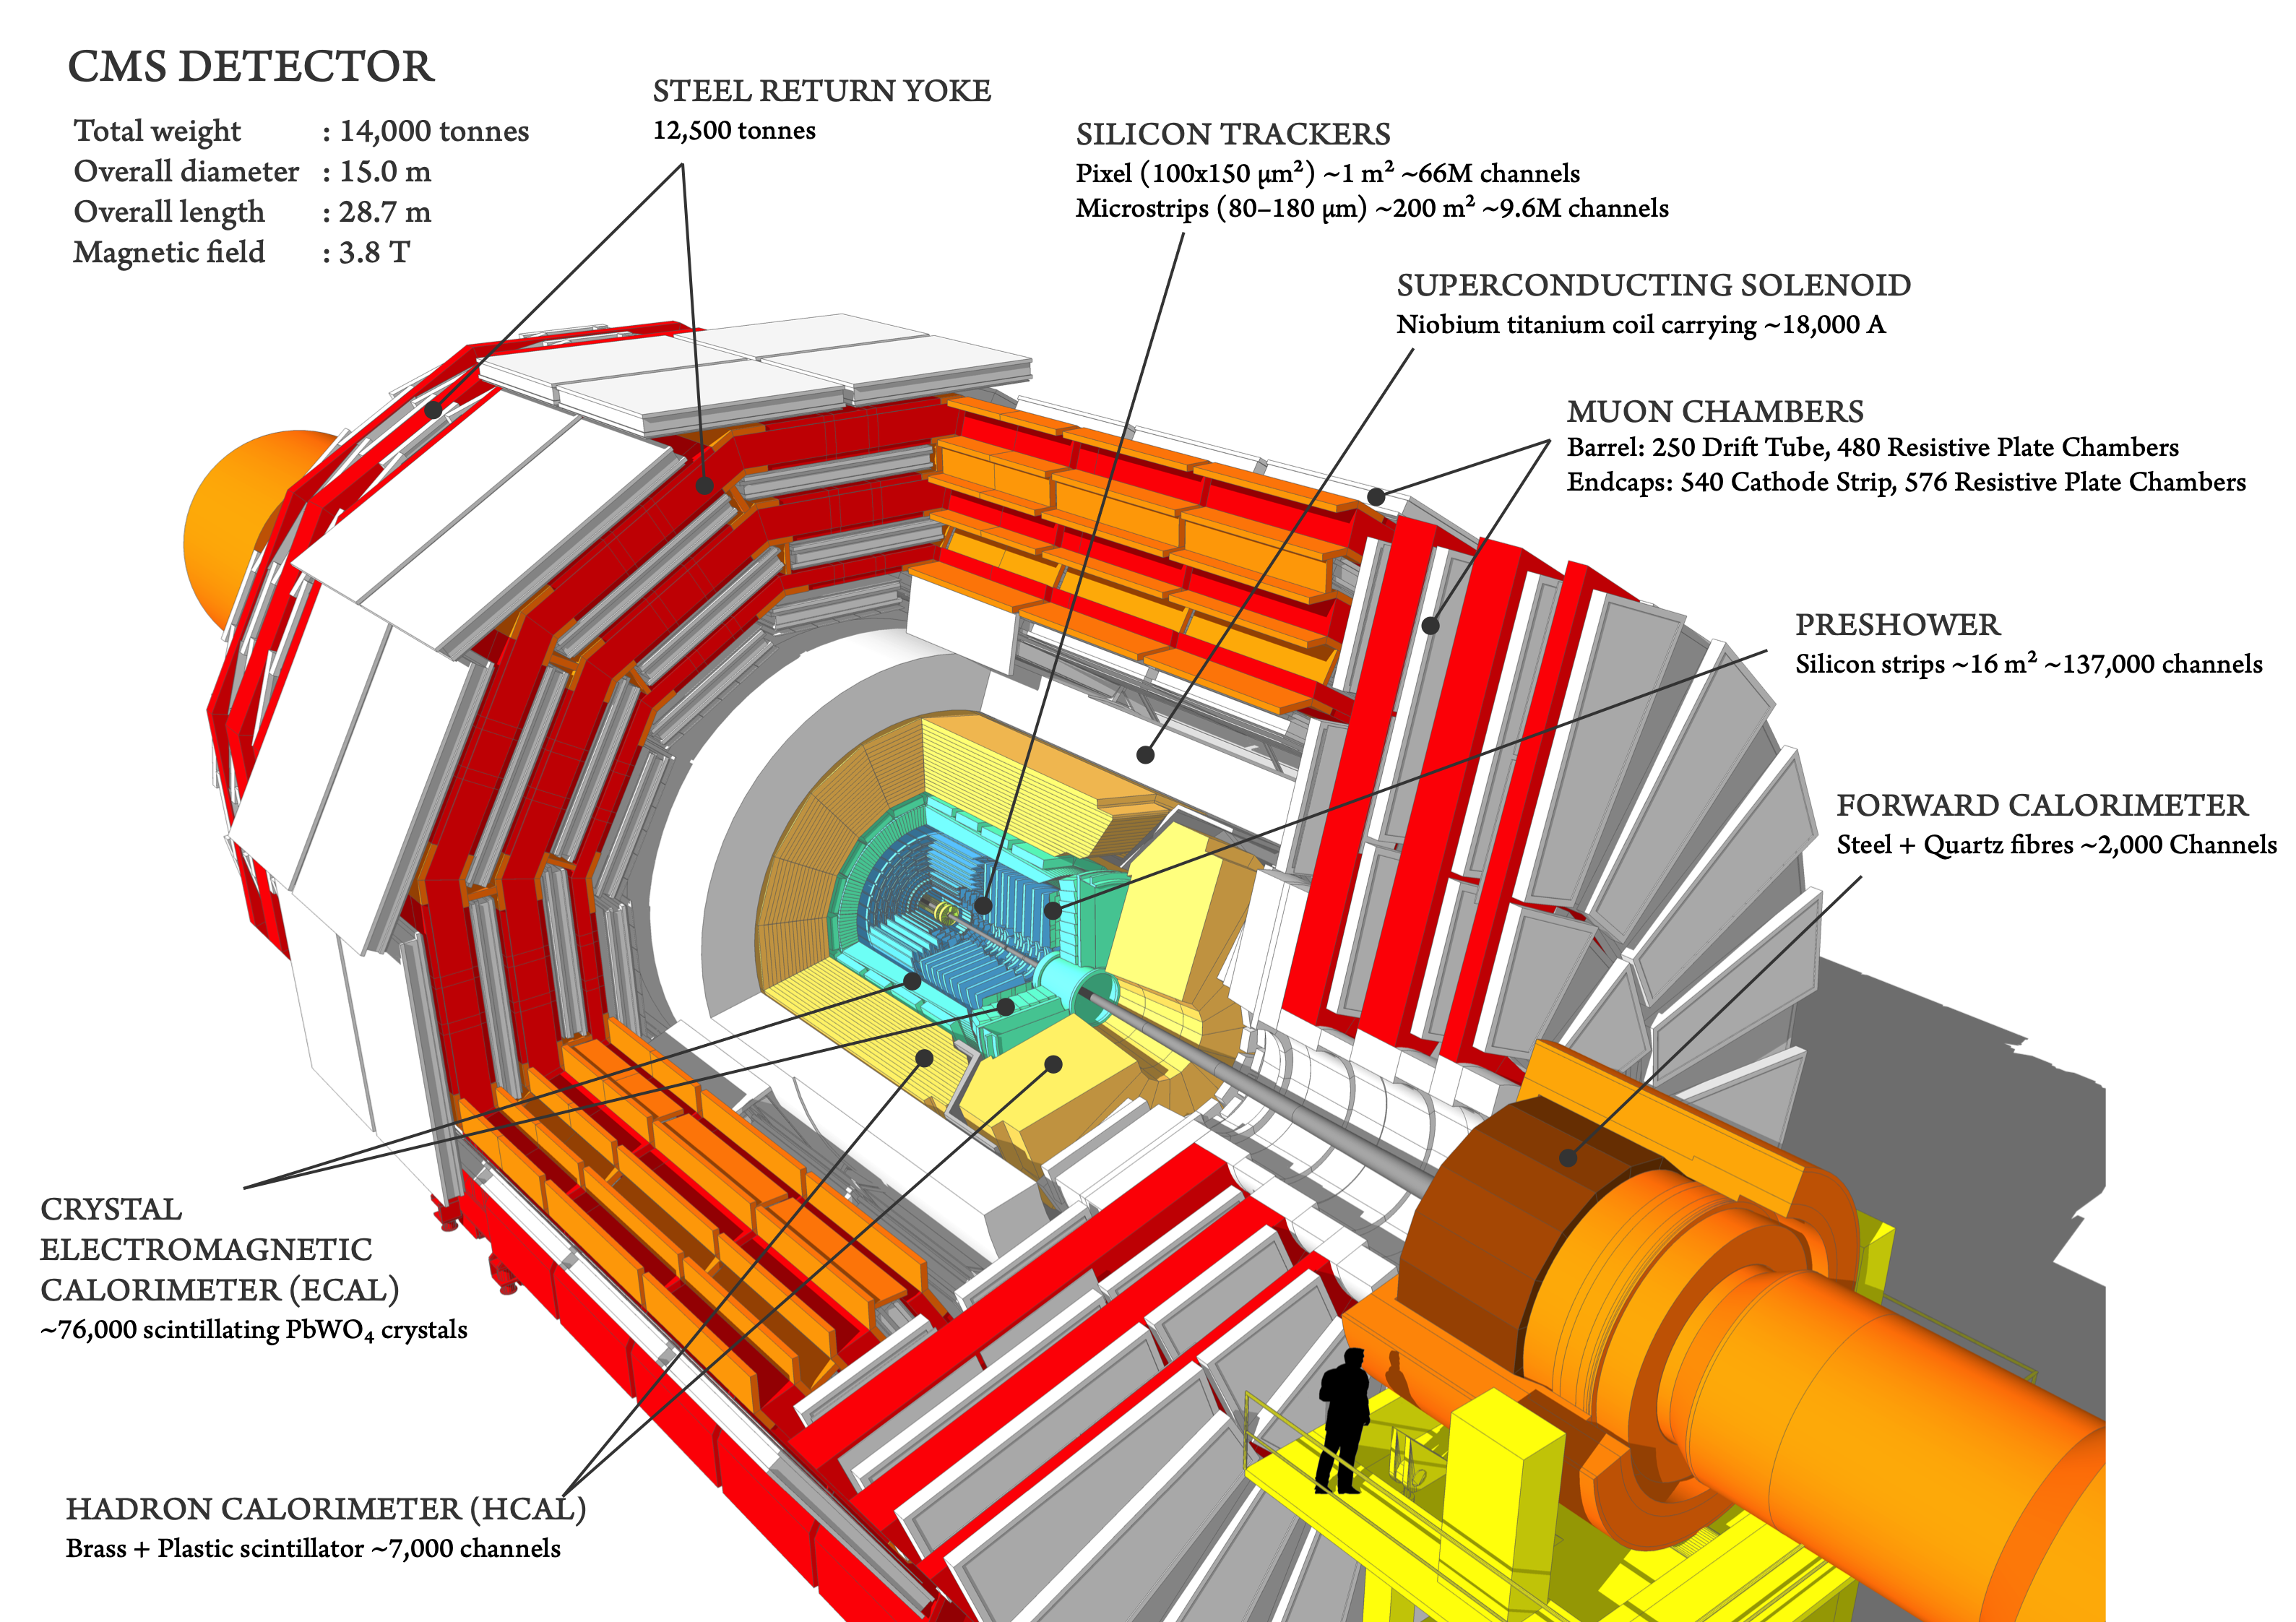
\includegraphics[width=1.0\linewidth]{images/CMS_disection_Run2.png}
    \caption{A schematic dissection of the CMS detector}
    \label{fig:CMS-disection}
\end{figure}

A defining characteristic of CMS is its powerful superconducting solenoid magnet with a inner bore of 5.9 meters and a length of 12.9 meters, capable of producing a magnetic field of 3.8 T inside its bore with a direction along the beam line, where the inner tracker and calorimeter modules are accommodated. The strong-magnetic-field design is in line with the demand for good momentum resolution within a relatively compact spectrometer.

Another distinctive advantage of CMS is its muon measurement capability, owing to its muon sub-detector module designs. With the return field of the superconducting solenoid strong enough to saturate 1.5 m of iron, the 4 muon "stations" are integrated inside the iron return yoke of the solenoid, providing a bending field of around 2 T and ensuring both robustness and full geometrical coverage. Each muon "station" consists of several layers of aluminium drift tubes (DT) in the barrel region and and cathode strip chambers (CSCs) in the endcap region, complemented by resistive plate chambers (RPCs). These detector modules work in tandem with the inner silicon tracker modules to produce a total reconstruction and identificaton efficiency of $> ~ 96\%$ and relative momentum resolution of $2\%$ for most muons and $10\%$ even for TeV muons.

\section{Dataset and Event Selection}

\subsection{Dataset}

In the present analysis, the dataset employed is the `ParkingDoubleMuonLowMass` collected from 2022 to 2024, all during the LHC Run 3 period, corresponding to a center-of-mass energy of $\sqrt{s} = 13.6 ~\text{TeV}$ and an integrated luminosity of $\mathcal{L}\approx176.6~\text{fb}^{-1}$.

\subsection{Triggering Condition}

The collision 

\subsection{Final State Particle Selection}

Given the excellent muon identification and measurement capability of the CMS detector,  we choose $J/\psi\to\mu^+\mu^-$ and $\Upsilon(nS)\to\mu^+\mu^-$ as the decay channel of these two heavy quarkonia. For $\phi$ mesons, the decay channel $\phi\to K^+K^-$ is chosen due to a relatively large branching ratio ($\approx 49\%$) \cite{PDG2020}.

In reconstruction of $\phi$ mesons, due to a relatively low identification ability for soft charged particles, all non-muon charged tracks are assumed to be $K^\pm$ and the tracks are paired only with the opposite-sign requirement.

Given that the transverse momenta of these final-state paticles typically fall in the $\text{GeV}$ region, the dominant background component for simultaneous production is the combinatorial background, with uncorrelated muons from $B$ and $D$ meson decays and light hadrons from soft-QCD processes.

To reduce background components, a further set of selection (shown in Table \ref{tab:mu_K_cuts}) is applied to the objects for event reconstruction.

\begin{table}[H]
    \centering
    \caption{Selection for final-state objects used in event reconstruction}
    \begin{tabular}{cl}
    \toprule
    Particle & Selection Criteria \\
    \midrule
    $\mu^\pm$ & Muon ID "soft" \\
              & $|\eta| < 2.4$ \\
              & $p_T > 3.5~\text{GeV/c}$ for $|\eta| < 1.2$ \\
              & $p_T > 2.5~\text{GeV/c}$ for $1.2 < |\eta| < 2.4$ \\
    Charged Tracks & High Purity \\
              & $|\eta|<2.5$ \\
              & $p_T > 2.0 ~\text{GeV/c}$ \\
    \bottomrule
    \end{tabular}
    \label{tab:mu_K_cuts}
\end{table}

To achieve a balance between signal-to-noise ratio and event statistics, we apply further individual selection for each process in the final signal extraction.

\section{Signal Extraction}

\section{Monte-Carlo (MC) Simulation Studies}

\section{Conclusions}



\begin{description}
  \item[$\bullet$]  What is the problem?
  \item[$\bullet$]  Why is it interesting and important?
  \item[$\bullet$]  Why is it hard? Why do naive approaches fail?
  \item[$\bullet$]  Why hasn't it been solved before? What's wrong with previous proposed solutions? How does mine differ?
  \item[$\bullet$]  What are the key components of my approach and results? Also include any specific limitations.
\end{description}
  
Then have a final paragraph or subsection: ``Summary of Contributions". It should list the major contributions in bullet form, mentioning in which sections they can be found. This material doubles as an outline of the rest of the paper, saving space and eliminating redundancy.

\section{Related Work}

The perennial question: Should related work be covered near the beginning of the paper or near the end?

\begin{description}
  \item[$\bullet$]  Beginning, if it can be short yet detailed enough, or if it's critical to take a strong defensive stance about previous work right away. In this case Related Work can be either a subsection at the end of the Introduction, or its own Section 2.
  \item[$\bullet$]  End, if it can be summarized quickly early on (in the Introduction or Preliminaries), or if sufficient comparisons require the technical content of the paper. In this case Related Work should appear just before the Conclusions, possibly in a more general section ``Discussion and Related Work".
\end{description}

\section{The Body}

\textbf{Guideline 1:} A clear new important technical contribution should have been articulated by the time the reader finishes page 3 i.e., a quarter of the way through the paper.

\textbf{Guideline 2:} Every section of the paper should tell a story. Don't, however, fall into the common trap of telling the entire story of how you arrived at your results. Just tell the story of the results themselves. The story should be linear, keeping the reader engaged at every step and looking forward to the next step. There should be no significant interruptions -- those can go in the Appendix.
\\
\\
Aside from these guidelines, which apply to every paper, the structure of the body varies a lot depending on content. Important components are:

\begin{description}
  \item[$\bullet$]  Running Example: When possible, use a running example throughout the paper. It can be introduced either as a subsection at the end of the Introduction, or its own Section 2 or 3 (depending on Related Work).
  \item[$\bullet$]  Preliminaries: This section, which follows the Introduction and possibly Related Work and/or Running Example, sets up notation and terminology that is not part of the technical contribution. One important function of this section is to delineate material that's not original but is needed for the paper. Be concise -- remember Guideline 1.
    \item[$\bullet$] Content: The meat of the paper includes algorithms, system descriptions, new language constructs, analyses, etc. Whenever possible use a ``top-down" description: readers should be able to see where the material is going, and they should be able to skip ahead and still get the idea.
\end{description}


\section{Performance Experiments}

We could have an entire treatise on this topic alone and I am surely not the expert. Here are some random thoughts:

\begin{description}
  \item[$\bullet$]  Many conferences expect experiments.
  \item[$\bullet$]  It's easy to do ``hokey" or meaningless experiments, and many papers do.
  \item[$\bullet$]  It's easy to craft experiments to show your work in its best light, and most papers do.
    \item[$\bullet$]  What should performance experiments measure? Possibilities:  
    \begin{description}
  	  \item[$\bullet$] Pure running time
      \item[$\bullet$] Sensitivity to important parameters
      \item[$\bullet$] Scalability in various aspects: data size, problem complexity, ...
  \end{description}
    \item[$\bullet$]  What should performance experiments show? Possibilities:
        \begin{description}
  	  \item[$\bullet$] Absolute performance i.e., it's acceptable/usable
      \item[$\bullet$] Relative performance to naive approaches
      \item[$\bullet$] Relative performance to previous approaches
      \item[$\bullet$] Relative performance among different proposed approaches
  \end{description}
  \item[$\bullet$] 
\end{description}


\section{The Conclusions}

In general a short summarizing paragraph will do, and under no circumstances should the paragraph simply repeat material from the Abstract or Introduction. In some cases it's possible to now make the original claims more concrete, e.g., by referring to quantitative performance results.

\section{Future Work}

This material is important -- part of the value of a paper is showing how the work sets new research directions. I like bullet lists here. A couple of things to keep in mind:
\begin{description}
  \item[$\bullet$]  If you're actively engaged in follow-up work, say so. E.g.: ``We are currently extending the algorithm to... blah blah, and preliminary results are encouraging." This statement serves to mark your territory.
\item[$\bullet$]  Conversely, be aware that some researchers look to Future Work sections for research topics. My opinion is that there's nothing wrong with that -- consider it a compliment.
\end{description}

\section{The Acknowledgements}

Don't forget them or you'll have people with hurt feelings. Acknowledge anyone who contributed in any way: through discussions, feedback on drafts, implementation, etc. If in doubt about whether to include someone, include them.


\section{Citations}

Spend the effort to make all citations complete and consistent. Do not just copy random inconsistent BibTex (or other) entries from the web and call it a day. Check over your final bibliography carefully and make sure every entry looks right.

\section{Appendix A}
This is a simple sample of a document created using \LaTeX
   (specifically pdflatex) that includes a figure from the Vergil visual editor for Ptolemy II
   that was created by printing to the Acrobat Distiller to get a PDF file.
   It also illustrates a simple two-column conference paper style,
   and use of bibtex to handle bibligraphies.

This is a sample document for use with pdflatex, which is
a program that is included with the Miktex distribution
that directly produces PDF files from \LaTeX sources.
To run \LaTeX on this file, you need the following files:
\begin{enumerate}
\item templatePDF.tex (this file)
\item figure.pdf (the figure file)
\item simpleConference.sty (style file)
\item refs.bib (bibiliography file)
\end{enumerate}
\noindent
To create a PDF file, execute the following commands:
\begin{enumerate}
\item pdflatex mainTemplatePDF
\item bibtex mainTemplatePDF
\item pdflatex mainTemplatePDF
\item pdflatex mainTemplatePDF
\end{enumerate}
\noindent
Yes (strangely) it is necessary to run pdflatex three times.
The result will be a PDF file (plus several other files that \LaTeX
produces).  You will need a mechanism, of course, for executing
commands on the command line. If you are using Windows, I recommend
installing Cygwin and using its bash shell.

\section{Appendix B: How to Include Vergil Diagrams as Figures}

\begin{figure}[!b]
  \begin{center}
    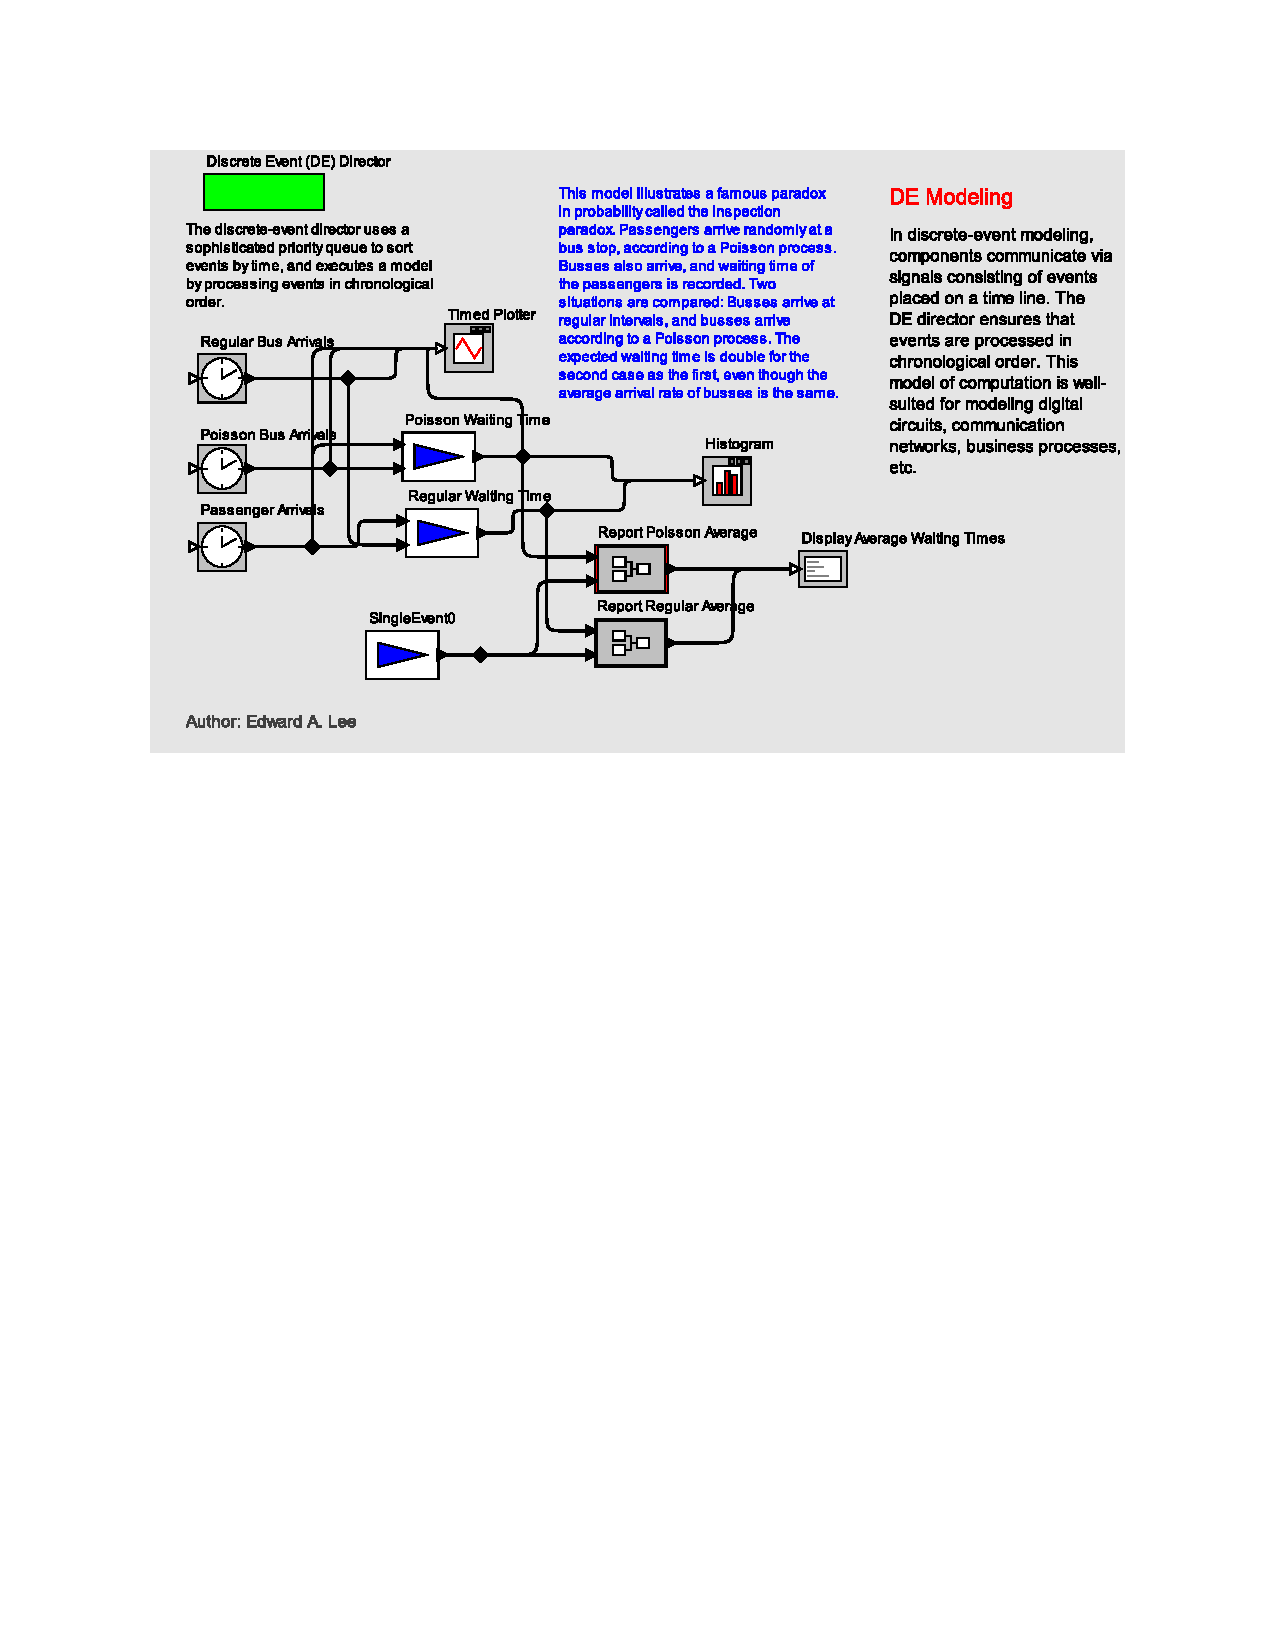
\includegraphics[width=3.5in]{figure.pdf}
  \end{center}

  \caption{\small Figure caption. To get a figure to span two
      columns, use the environment figure* rather than figure.}
  \label{fig-label}
\end{figure}

\begin{figure*}[!b]
  \begin{center}
    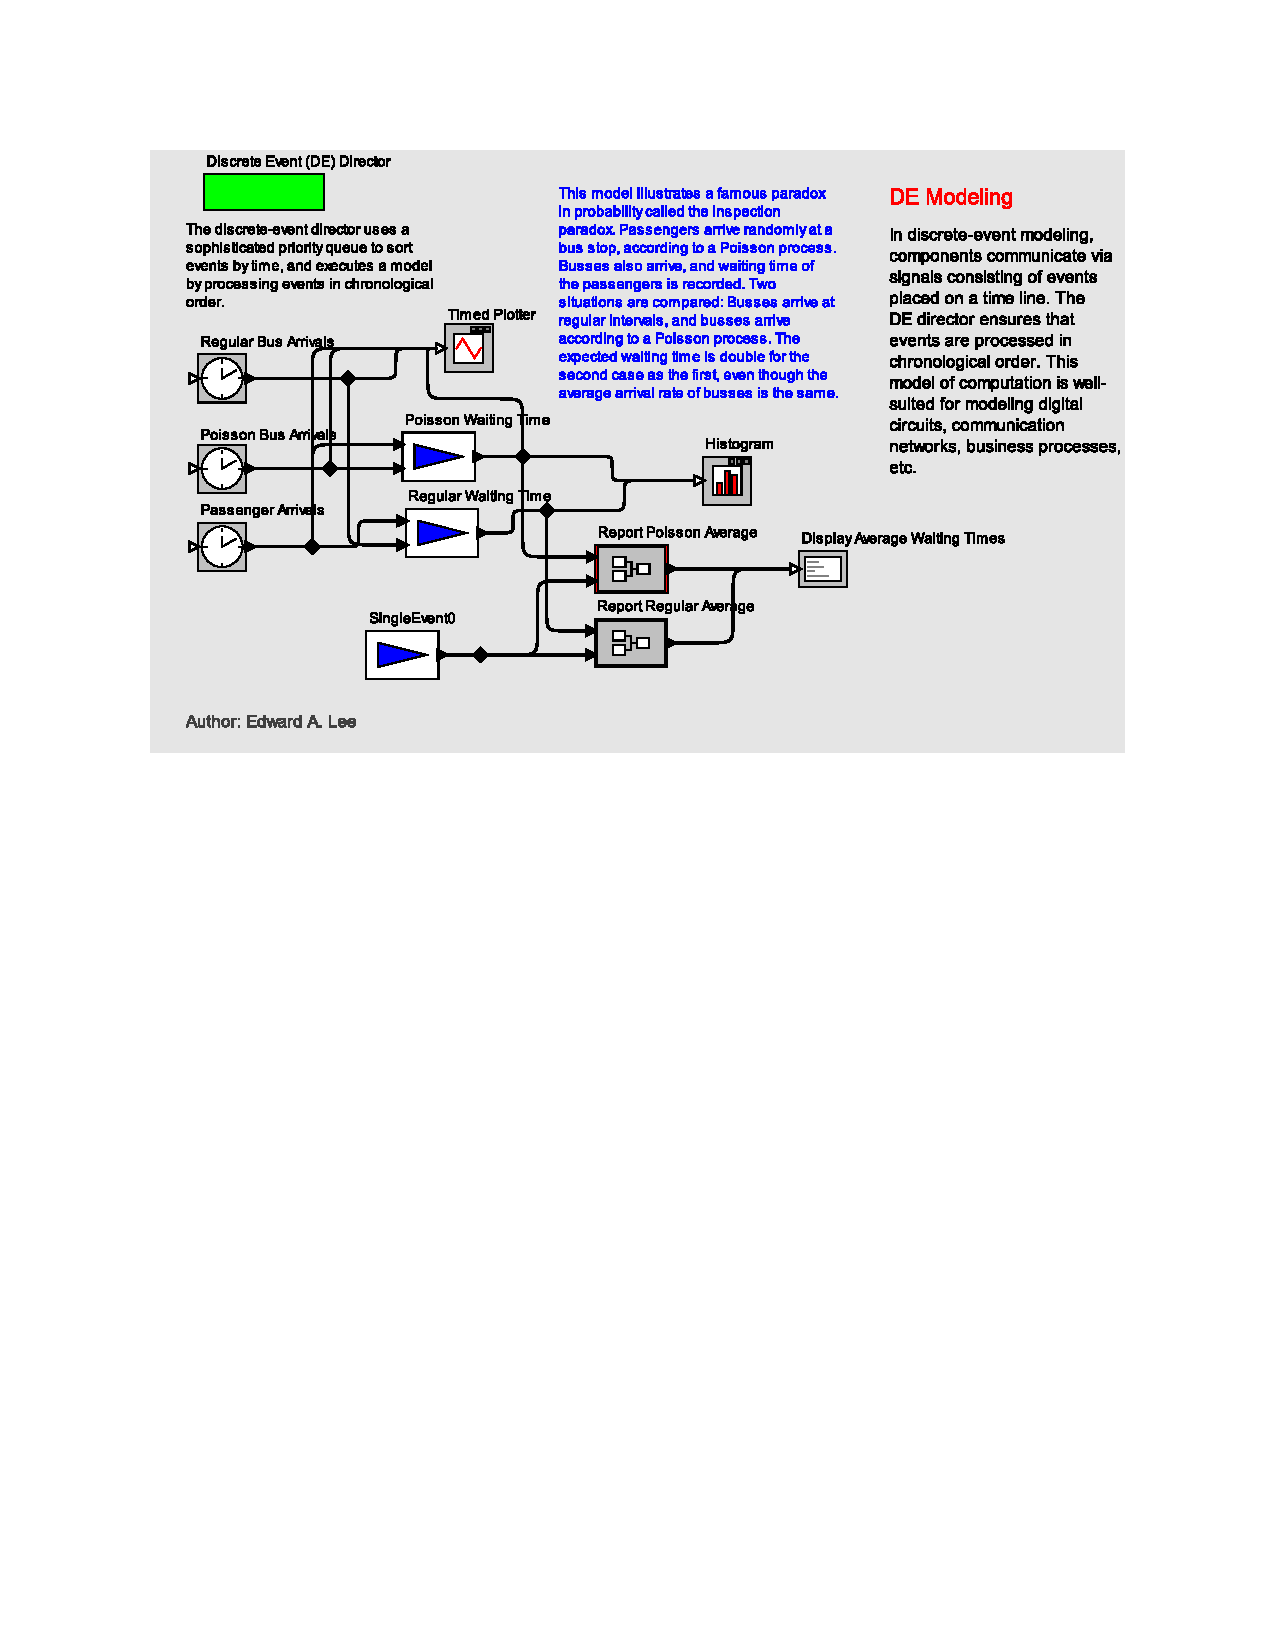
\includegraphics[width=3.5in]{figure.pdf}
  \end{center}

  \caption{\small Figure caption. To get a figure to span two
      columns, use the environment figure* rather than figure.}
  \label{fig-label}
\end{figure*}

Suppose you wish to include a figure, like that in figure \ref{fig-label}.
The simplest mechanism is to install Adobe Acrobat, which includes
a ``printer'' called ``Acrobat Distiller.'' Printing to this printer
creates a PDF file, which can be included in a document as shown
here.  To include Ptolemy II models \cite{PtolemyVol1:04},
just print to the distiller from within Vergil and reference
the PDF file in your \LaTeX document.

There is a bit more work to do, however.
The file that is produced by the distiller represents
a complete page, not the individual figure.
You can open it in using Acrobat (version 5.0 or later),
and select Document $\to$ Crop Pages from the menu.
In the resulting dialog, check ``Remove White Margins.''
Save the modified PDF file in a file and then reference
it in the \LaTeX file as shown in this example.

An alternative is to generate EPS (encapsulated postscript),
but the process is much more complex and fragile.
I recommend using pdflatex and Adobe Acrobat.

\bibliographystyle{abbrv}
\bibliography{refs}
\end{document}
